
\thispagestyle{empty}
\begin{figure}[h]
\centering
 
\includegraphics[width=12cm]{fig/logo.png} % leia abaixo
\label{figura:abobora}
\end{figure}

\begin{center}
     {\large {\textbf 
    6º Abóbora Contest \& 3ª Maratona de Programação IF}}
    
    %Sub-Regional Brasil do ACM ICPC
    {\large 30 de Setembro de 2025}   
    
    {\large \textbf{Instruções para uso do sistema de submissão Boca}}
\end{center}
Adaptado de ICPC Latin American Regional Contests, 2024.
\begin{enumerate}
    \item \textbf{Esclarecimentos (\textit{clarifications})}
    
    Toda a comunicação com os juizes é feita através das mensagens de \textbf{esclarecimentos}. Para solicitar um esclarecimento sobre algum problema você deverá utilizar a interface \textit{web} do Boca:
    \begin{enumerate}
        \item Abra seu navegador;
        \item Efetue login como time;
        \item Acesse a opção \textit{clarifications}. Escolha o problema sobre o qual você necessita esclarecimento, digite sua pergunta e submeta.
    \end{enumerate}
    Tanto os pedidos de esclarecimento enviados por vocês quanto as respostas dos juízes estarão disponíveis nessa mesma tela. Haverá um alerta pela interface \textit{web} sempre que você obtiver resposta para algum pedido de esclarecimento. Caso o juiz entenda que o seu esclarecimento se aplica aos demais, será feito um esclarecimento global.
    \item \textbf{Placar (\textit{score board})}
    
    Para visualizar o placar (\textit{score board}), onde você poderá acompanhar o \textit{ranking} entre os times, você deverá utilizar a interface \textit{web} do Boca:
    \begin{enumerate}
        \item Abra seu navegador;
        \item Efetue login como time;
        \item Acesse a opção \textit{Score}. Você terá acesso ao \textit{ranking} completo.
    \end{enumerate}
    \item \textbf{Tarefas (\textit{tasks})}
    
    A aba \textit{Tasks} permite que o time envie códigos para impressão, bem como solicitar ajuda de algum membro do suporte (\textit{staff}).
    \begin{enumerate}
        \item Abra seu navegador;
        \item Efetue login como time e vá até a aba \textit{Tasks};
        \item Para imprimir um arquivo selecione ele no disco e clique em enviar (\textit{Send});
        \item Para solicitar ajuda, clique no botão \textit{S.O.S.}. Note que a ajuda feita pelo suporte terá relação \textit{apenas} com problemas na máquina ou outro problema físico.
    \end{enumerate}
\end{enumerate}

\newpage

\include{abobora_25/regras25}
\begin{center}
Problema A

Caminho da Colheita

{\small Nome do arquivo: A.c, A.cpp, A.java, ou A.py}

{\large Timelimit: $1$}

{\tiny Por Athos José}

\end{center}

Seu Zé, fazendeiro importante de Rio Verde tem uma plantação de abóboras organizadas em uma área retangular de tamanho $N$ x $M$, cada muda de abóbora está em uma área $1$x$1$ e contém uma certa quantidade de abóboras.

Costumeiramente, Seu Zé faz a colheita em um percurso único, começando no canto superior esquerdo do campo (posição ($1,1$)) e termina sempre no canto inferior direito do campo ($N,M$). A cada passo, ele mover-se apenas para a direita ou para baixo.

A plantação de Seu Zé cresceu muito e acredita que o carinho que usa para colher não é suficientemente grande para acomodar todas as abóboras no caminho. Agora ele pediu sua ajuda para que dado o campo informa-se qual é máximo de abóboras possível de colher ao longo do melhor caminho.

\vspace{0.3cm}
\begin{figure}[h]
    \centering
    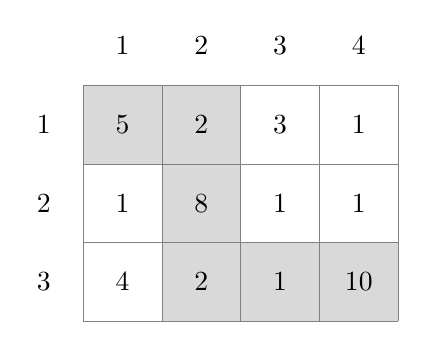
\begin{tikzpicture}
        \fill[gray!30] (0,2) rectangle (1,3);
        \fill[gray!30] (1,2) rectangle (2,3);
        \fill[gray!30] (1,1) rectangle (2,2);
        \fill[gray!30] (1,0) rectangle (2,1);
        \fill[gray!30] (2,0) rectangle (3,1);
        \fill[gray!30] (3,0) rectangle (4,1);

        \draw[gray,very thin] (0,0) grid (4, 3);

        \node at (0.5, 2.5) {5};
        \node at (1.5, 2.5) {2};
        \node at (2.5, 2.5) {3};
        \node at (3.5, 2.5) {1};

        \node at (0.5, 1.5) {1};
        \node at (1.5, 1.5) {8};
        \node at (2.5, 1.5) {1};
        \node at (3.5, 1.5) {1};

        \node at (0.5, 0.5) {4};
        \node at (1.5, 0.5) {2};
        \node at (2.5, 0.5) {1};
        \node at (3.5, 0.5) {10};

        \node at (1.5, 3.5) {2};
        \node at (0.5, 3.5) {1};
        \node at (2.5, 3.5) {3};
        \node at (3.5, 3.5) {4};

        \node at (-0.5, 2.5) {1};
        \node at (-0.5, 1.5) {2};
        \node at (-0.5, 0.5) {3};
    \end{tikzpicture}
    \caption{Exemplo da entrada com células coloridas}
\end{figure}

\vspace{0.3cm}
\textbf{Entrada}

A primeira linha contém dois inteiros $N$ e $M$ ($1 \leq N, M \leq 2000$), representando respectivamente o número de linhas e colunas da grade.

Em seguida, seguem $N$ linhas, cada uma contendo $M$ inteiros $C_{i,j}$ ($0 \leq C_{i,j} \leq 10^4$), representando a quantidade de abóboras em cada posição $i$ e $j$.

\vspace{0.3cm}
\textbf{Saída}

Imprima um único inteiro, sendo o número máximo de abóboras que podem ser colhidas seguindo as regras.

\begin{table}[ht]
    \centering
    \begin{tabular}{|p{7cm}|p{7cm}|}
        \hline
        \begin{center}
            \vspace{-0.3cm}
            \textbf{Exemplos de Entrada}
            \vspace{-0.3cm}
        \end{center} 
         &  
        \begin{center}
            \vspace{-0.3cm}
            \textbf{Exemplos de Saída}
            \vspace{-0.3cm}
        \end{center} \\ \hline
         \texttt{3 4} & \texttt{28} \\
         \texttt{5 2 3 1} & \texttt{} \\
         \texttt{1 8 1 1} & \texttt{} \\
         \texttt{4 2 1 10} & \texttt{} \\
         \hline
    \end{tabular}
    
    \caption{Exemplos de entradas e saídas}
    \label{tab:inputA1}
    
\end{table}

\vspace{0.3cm}

\newpage

\begin{center}
\noindent
\lstinputlisting{abobora_25/A/A5.cpp}
\end{center}
\begin{center}
Problema B

O Desafio do Chocolate do Zé do Grafo

{\small Nome do arquivo: B.c, B.cpp, B.java, ou B.py}

{\large Timelimit: $1$}

{\tiny Por André da Cunha Ribeiro}

\end{center}					

Todo competidor de maratona de programação sabe que as longas horas de um concurso exigem um combustível especial para o cérebro. E qual é o lanche preferido de 10 entre 10 programadores para manter o foco e a energia? Chocolate, é claro! A combinação de açúcar e cafeína parece ter sido feita sob medida para transformar um bug teimoso em um cobiçado "Accepted".

%Zé do Grafo, mais do que um professor, é um mentor que entende perfeitamente a rotina de seus alunos. Vendo sua equipe exausta após um treino intenso para a grande final da competição, ele aparece com o suprimento de energia definitivo: uma enorme barra de chocolate retangular, com N fileiras e M colunas.

%Mas, fiel ao seu estilo, Zé do Grafo não perderia a chance de um bom desafio. Ele colocou a barra de chocolate sobre a mesa e continuou: "O processo para dividir nosso prêmio é simples. A cada movimento, só podemos pegar um único pedaço de chocolate e quebrá-lo uma única vez, sempre em linha reta, seguindo um dos sulcos que dividem os quadrados. Cada quebra transforma um pedaço em dois. Vamos repetir isso até que toda a barra se transforme nos pequenos quadrados individuais de 1x1."

%Ele fez uma pausa e olhou para a equipe com um olhar astuto. "Agora, a pergunta que vale o primeiro pedaço: qual o número exato de quebras necessárias para completar a tarefa?"


Zé do Grafo, um famoso professor de Teoria dos Grafos e um ávido criador de quebra-cabeças, propôs um desafio para seus alunos. Ele apresentou uma barra de chocolate retangular, dividida em pequenos quadrados por sulcos, formando uma grade de $N$ fileiras e $M$ colunas.

O desafio é o seguinte: para dividir a barra de chocolate em $(N * M)$ quadrados de chocolate individuais, os alunos só podem realizar um tipo de movimento. A cada passo, eles podem pegar um único pedaço de chocolate e quebrá-lo ao longo de um dos sulcos (seja na horizontal ou na vertical), resultando em dois pedaços menores.

Sua tarefa é criar um programa que ajude os alunos do Zé do Grafo a descobrir rapidamente o número total de quebras necessárias para transformar a barra inteira em quadrados individuais.

\vspace{0.3cm}
\textbf{Entrada}
A entrada contém  na primeira linha o valor $1 \leq X \leq 1000$ que representa o número dos casos de teste. Seguido de $X$ leituras dos valores de $N,M$ $(1 \leq N,M \leq 10^9)$ indicando as dimensões dos chocolates. 


\vspace{0.3cm}
\textbf{Saída}
Para cada caso de teste, o programa deve produzir uma linha na saída, contendo um único inteiro que representa o número total de quebras necessárias para dividir o chocolate daquele caso de teste.

{\tiny
\begin{table}[h]
    \centering
    \begin{tabular}{|p{7cm}|p{7cm}|}
        \hline
        \begin{center}
            \vspace{-0.3cm}
            \textbf{Exemplos de Entrada}
            \vspace{-0.3cm}
        \end{center} 
         &  
        \begin{center}
            \vspace{-0.3cm}
            \textbf{Exemplos de Saída}
            \vspace{-0.3cm}
        \end{center} \\ \hline
         \texttt{4} & \texttt{3} \\  
         \texttt{2 2} & \texttt{23} \\
         \texttt{4 6} & \texttt{55} \\
         \texttt{7 8} & \texttt{836} \\
         \texttt{27 31} & \texttt{} \\
        \hline
    \end{tabular}
    \caption{Exemplos de entradas e saídas}
\end{table}}

\newpage

\begin{center}
\noindent
\lstinputlisting{abobora_25/B/B5.cpp}
\end{center}

\begin{center}
Problema C

Otimização de Rotas de Coleta de Solo - Simple Smart Agro

{\small Nome do arquivo: C.c, C.cpp, C.java, ou C.py}

{\large Timelimit: $2$}

{\tiny Por Alexandre da Silva}

\end{center}	

\footnotesize
			
A Simple Smart Agro está desenvolvendo um sistema automatizado para coleta de amostras de solo em uma fazenda. O sistema precisa otimizar as rotas de coleta para maximizar a eficiência do processo. Existem $N$ pontos específicos onde amostras de solo devem ser coletadas. O veículo de coleta parte sempre do depósito localizado na origem $(0, 0)$ e deve retornar ao mesmo ponto após coletar todas as amostras. Devido às características do terreno e dos equipamentos, o veículo só pode se mover nas direções cardeais (norte, sul, leste, oeste) e sempre em linha reta entre dois pontos consecutivos da rota. A distância entre dois pontos $(x_1, y_1)$ e $(x_2, y_2)$ é calculada usando a distância Manhattan: $|x_1 - x_2| + |y_1 - y_2|$.

\subsection*{Entrada}

\begin{itemize}
    \item A primeira linha contém um inteiro $N$ $(1 \leq N \leq 10)$, representando o número de pontos de coleta;
    \item As próximas $N$ linhas contêm dois inteiros $x_i$ e $y_i$ $(-1000 \leq x_i, y_i \leq 1000)$, representando as coordenadas do $i$-ésimo ponto de coleta;
       \item Todos os pontos de coleta são distintos entre si;
    \item Nenhum ponto de coleta coincide com a origem $(0,0)$.
\end{itemize}

\subsection*{Saída}

\begin{itemize}
    \item Uma única linha contendo um inteiro: a menor distância total (distância Manhattan) necessária para visitar todos os pontos de coleta e retornar à origem.
\end{itemize}

\subsection*{Exemplos}

\begin{center}
\begin{tabular}{|p{6cm}|p{4cm}|}
\hline
\textbf{Exemplo de Entrada} & \textbf{Exemplo de Saída} \\
\hline
\texttt{3} & \texttt{26} \\
\texttt{2 3} & \\
\texttt{7 1} & \\
\texttt{5 6} & \\
\hline
\texttt{4} & \texttt{42} \\
\texttt{3 4} & \\
\texttt{8 2} & \\
\texttt{12 8} & \\
\texttt{6 10} & \\
\hline
\texttt{1} & \texttt{8} \\
\texttt{2 2} & \\
\hline
\end{tabular}
\end{center}

\subsection*{Explicação do Primeiro Exemplo}

Partindo da origem $(0,0)$, temos os pontos de coleta em $(2,3)$, $(7,1)$ e $(5,6)$.
Uma rota ótima seria:
$(0,0) \rightarrow (2,3) \rightarrow (5,6) \rightarrow (7,1) \rightarrow (0,0)$

Calculando as distâncias:
\begin{itemize}
    \item $(0,0)$ para $(2,3)$: $|2-0| + |3-0| = 2 + 3 = 5$
    \item $(2,3)$ para $(5,6)$: $|5-2| + |6-3| = 3 + 3 = 6$
    \item $(5,6)$ para $(7,1)$: $|7-5| + |1-6| = 2 + 5 = 7$
    \item $(7,1)$ para $(0,0)$: $|0-7| + |0-1| = 7 + 1 = 8$
\end{itemize}

Distância total: $5 + 6 + 7 + 8 = 26$


\newpage

\begin{center}
\noindent
\lstinputlisting{abobora_25/C/C5.cpp}
\end{center}
\begin{center}
Problema D

Agência de Espionagem

{\small Nome do arquivo: D.c, D.cpp, D.java, ou D.py}

{\large Timelimit: $1$}

{\tiny Por Athos José}


\end{center}

A Agência Nacional de Espionagem mantém em seus cofres uma coleção de símbolos secretos, representados por uma sequência de letras. Esses símbolos podem ser reorganizados em qualquer ordem, de forma a formar novas mensagens.

Agentes inimigos, porém, estão tentando criar mensagens escondidas dentro dessas reorganizações. Uma mensagem inimiga é considerada possível se puder aparecer como uma sequência contínua de caracteres de alguma permutação dos símbolos guardados no cofre.

Sua missão é, para cada mensagem inimiga recebida, determinar se ela pode ser formada a partir dos símbolos da Agência.

\vspace{0.3cm}
\textbf{Entrada}

A primeira linha contém um inteiro $N$ ($1 \leq N \leq 10^5$), o número de mensagens inimigas a serem analisadas, seguido de uma string $S$ ($1 \leq |S| \leq 10^5$) representando os símbolos secretos do cofre.

Cada uma das próximas $N$ linhas contém uma string $Q_i$ ($1 \leq |Q_i| \leq 10^5$), representando uma mensagem inimiga a ser verificada.

A soma dos comprimentos de todas as mensagens $Q_i$ não excede $10^9$.

Todas as strings são compostas apenas de letras minúsculas do alfabeto inglês (a-z).

\vspace{0.3cm}
\textbf{Saída}

Para cada mensagem $Q_i$ imprima uma linha contendo:
\begin{itemize}
    \item ``SIM'', se a mensagem pode ser formada como substring de alguma permutação de $S$.
    \item ``NAO'',caso contrário.
\end{itemize}

\begin{table}[h]
    \centering
    \begin{tabular}{|p{7cm}|p{7cm}|}
       \hline
        \begin{center}
            \vspace{-0.3cm}
            \textbf{Exemplos de Entrada}
            \vspace{-0.3cm}
        \end{center} 
         &  
        \begin{center}
            \vspace{-0.3cm}
            \textbf{Exemplos de Saída}
            \vspace{-0.3cm}
        \end{center} \\ \hline
         \texttt{3 abac} & \texttt{SIM} \\  
         \texttt{caa} & \texttt{NAO} \\
         \texttt{aaa} & \texttt{SIM} \\  
         \texttt{bac} & \\
         \hline
    \end{tabular}
    \caption{Exemplos de entradas e saídas}
    \label{tab:inputB}
\end{table}

\newpage

\begin{center}
\noindent
\lstinputlisting{abobora_25/D/D5.cpp}
\end{center}
\begin{center}
Problema E

Estória da Estônia

{\small Nome do arquivo: E.c, E.cpp, E.java, ou E.py}

{\large Timelimit: $1$}

{\tiny Por Márcio Belo}

\end{center}			

O professor Márcio Belo sempre gostou de charadas matemáticas. Um dia ele se deparou com uma estória, pra lá da Estônia. Dado um número primo ímpar $p$, sempre é possível um triângulo de lados inteiros $x$, $y$ e $z$, em ordem crescente de tamanho com as seguintes propriedades: 
\begin{itemize}
    \item A diferença da soma dos lados menores do triângulo pelo lado maior é igual ao primo $p$; 
    \item A diferença da soma das áreas dos quadrados de lados $x$ e $y$ e a área do quadrado de lado $z$ é igual ao primo $p$. 
\end{itemize}
Em matematiquês:

\vspace{3mm}
Dado um primo $p \geq 3$, sempre existem triplas $(x,y,z)$, com $x \leq y \leq z$ que satisfazem: 
\begin{align*}
    x + y - z & = p \\
    x^{2} + y^{2} - z^{2} & = p 
\end{align*}
Quem são essas triplas $(x,y,z)$? Você pode ajudar o professor?

\vspace{0.3cm}
\textbf{Entrada}
Cada entrada contém uma única linha com o número primo $p$, com $(3 \leq p < 2^{16})$. 

\vspace{0.3cm}
\textbf{Saída}
O sistema deve retornar todas as triplas $(x,y,z)$ em ordem crescente de $x$. Uma tripla por linha,  

\begin{table}[h]
    \centering
    \begin{tabular}{|p{7cm}|p{7cm}|}
        \hline
        \begin{center}
            \vspace{-0.3cm}
            \textbf{Exemplos de Entrada}
            \vspace{-0.3cm}
        \end{center} 
         &  
        \begin{center}
            \vspace{-0.3cm}
            \textbf{Exemplos de Saída}
            \vspace{-0.3cm}
        \end{center} \\ \hline
         \texttt{3} & \texttt{(4,6,7)} \\  
         \hline
         \texttt{5} & \texttt{(6, 15, 16)} \\ 
          & \texttt{(7, 10, 12)} \\ 
         \hline
         \texttt{13} & \texttt{(14, 91, 92)} \\
         & \texttt{(15, 52, 54)} \\
         & \texttt{(16, 39, 42)} \\
         & \texttt{(19, 26, 32)} \\ 
         \hline
         \texttt{65267} & \texttt{(65268,2129923278,2129923279)} \\ 
          & \texttt{(97900,130534,163167)} \\ 
         \hline
    \end{tabular}
    \caption{Exemplos de entradas e saídas}

\end{table}

\newpage
\begin{center}
\noindent
\lstinputlisting{abobora_25/E/E5.cpp}
\end{center}
\begin{center}
Problema F

Monitorando Pragas

{\small Nome do arquivo: F.c, F.cpp, F.java, ou F.py}

{\large Timelimit: $1$}

{\tiny Por Emanuel Silva Araujo}

\end{center}

\footnotesize

O agricultor Seu Jayme sofre constantemente com infestações de insetos em sua lavoura de soja. Para reduzir perdas e otimizar o manejo, ele procurou a EMBRAPII para desenvolver uma ferramenta de monitoramento diário de pragas.
Sua tarefa como programador é implementar um programa que leia os valores de população diária e identifique situações de risco, emitindo alertas de acordo com os seguintes critérios:
%Critérios de Alerta
    \begin{itemize}
        \item  Alerta por pico diário [Pico]
        \begin{itemize}
            \item Se em qualquer dia a população registrada ultrapassar 200 insetos.
        \end{itemize}
        \item  Alerta por variação em 7 dias [7 Dias]
        \begin{itemize}
            \item Se a diferença percentual entre o valor mínimo e o máximo em um intervalo de 7 dias consecutivos for maior ou igual a 20\%.
        \end{itemize}
        \item  Alerta por crescimento contínuo [Crescimento]
        \begin{itemize}
            \item Se ocorrerem 4 dias seguidos de crescimento, e em cada dia a população for pelo menos 5\% maior que a do dia anterior.
        \end{itemize}
    \end{itemize}
        
\vspace{0.3cm}
\textbf{Entrada}

Um número inteiro $(0 <= N <= 360)$, representando a quantidade de dias monitorados (entre os dias $0$ e $360$).
Uma sequência de $N$ números inteiros $(0 < X <= 5000)$, cada um representando a estimativa da população de insetos no respectivo dia.

\vspace{0.3cm}
\textbf{Saída}

    Para cada alerta identificado, o programa deve imprimir:
    \begin{itemize}
        \item O tipo do alerta;
        \item O(s) dia(s) correspondente(s);
        \item O valor percentual (quando aplicável), com duas casas decimais.
    \end{itemize}
    Caso não tenha nenhum alerta, deve imprimir uma mensagem de "Nenhum Alerta".
    Para dias que tiveram mais de um alerta a ordem de impressão é: $[Pico] > [7 Dias] > [Crescimento]$.
 
\begin{table}[h]
    \centering
    \footnotesize
    \begin{tabular}{|p{8cm}|p{8cm}|}
        \hline
        \begin{center}
            \vspace{-0.3cm}
            \textbf{Exemplos de Entrada}
            \vspace{-0.3cm}
        \end{center} 
         &  
        \begin{center}
            \vspace{-0.3cm}
            \textbf{Exemplos de Saída}
            \vspace{-0.3cm}
        \end{center} \\ \hline
		    \texttt{10} & \texttt{[Crescimento] 1-4: maior que >= 5\% } \\
                \texttt{50 60 70 80 90 200 210 220 180 170} & \texttt{[Crescimento] 1-5: maior que >= 5\% } \\
& \texttt{[Crescimento] 1-6: maior que >= 5\% } \\
& \texttt{[Pico] 7: 210 insetos} \\
& \texttt{[7 Dias] 1-7: 320.00\%} \\
& \texttt{[Crescimento] 1-7: maior que >= 5\% } \\
& \texttt{[Pico] 8: 220 insetos} \\
& \texttt{[7 Dias] 2-8: 266.67\%} \\
& \texttt{[7 Dias] 3-9: 214.29\%} \\
& \texttt{[7 Dias] 4-10: 175.00\%} \\


         \hline
   		    \texttt{9}   & \texttt{[Crescimento] 1-4: maior que >= 5\% } \\
            \texttt{100 105 112 118 90 96 100 120 80} & \texttt{[7 Dias] 2-8: 33.33\%} \\
         \hline    
   		    \texttt{8}   & \texttt{Nenhum Alerta} \\
            \texttt{118 120 118 140 140 140 130 100} & \\
         \hline    
    \end{tabular}
    \caption{Exemplos de entradas e saídas}

\end{table}

\normalsize

\newpage

\begin{center}
\lstinputlisting{abobora_25/F/F5.cpp}
\end{center}

\begin{center}
Problema G

Comportamento Dinâmico

{\small Nome do arquivo: G.c, G.cpp, G.java, ou G.py}

{\large Timelimit: $1$}

{\tiny Por Heverton Barros de Macêdo}

\end{center}

\footnotesize

	Durante uma investigação sobre o comportamento de sistemas dinâmicos, Wolfram definiu o seguinte cenário para efetuar experimentos: dada uma cadeia de $N$ células, linearmente distribuídas, cada célula armazena um único estado (bit), e além disso as células das extremidades são vizinhas entre si. Para cada instante de tempo $t$ a evolução dessa cadeia ocorre simultaneamente em todas as células, considerando uma regra de evolução previamente definida. Essa regra é aplicada a cada vizinhança de $K=3$ células gerando um novo estado, conforme indicado na Tabela~\ref{tab:evolucao}.
	
	\begin{table}[h!]
		\caption{Regra aplicada para evolução do experimento de Wolfram.}
		\label{tab:evolucao}
		
		\centering
		\footnotesize{
		\begin{tabular}{|c|c|c|c|c|c|c|c|c|}
			\hline
			\cellcolor[HTML]{DDDDDD} Regra para vizinhança & 000 & 001 & \cellcolor[HTML]{FFAAAA} 010 & 011 & 100 & 101 & 110 & 111 \\ \hline
			\cellcolor[HTML]{DDDDDD} Novo estado para célula central & 1 & 0 &  \cellcolor[HTML]{AAFFAA} 0 & 1 & 0 & 0 & 0 & 1 \\ \hline
		\end{tabular}
		}
	\end{table}

Como exemplo, considere um experimento (veja a Tabela~\ref{tab:exemplo_evolucao}) com a cadeia de bits formada por $11$ células ($N = 11$), em que no instante $t = 0$ apenas um bit, exatamente no centro da cadeia, possui o estado $1$ e as demais células possuem o estado $0$, evoluindo por $4$ passos de tempo ($t = 4$).
%Como exemplo, considere um experimento (veja a Tabela~\ref{tab:exemplo_evolucao}) com a cadeia de bits no espaço linear formada por $11$ células ($N = 11$), em que apenas um bit, exatamente no centro da cadeia ($t = 0$), possui o estado $1$ e as demais células possuem o estado $0$, evoluindo por $4$ passos de tempo.

A Tabela~\ref{tab:exemplo_evolucao} ilustra o experimento com a configuração inicial ($t = 0$) formada por: $00000100000$. No próximo passo de tempo ($t = 1$), todas as células evoluem (podem alterar o estado) considerando a vizinhança indicada na regra (Tabela~\ref{tab:evolucao}). Em destaque na cor vermelha (Tabelas~\ref{tab:evolucao} e ~\ref{tab:exemplo_evolucao}) está a atualização da célula central, formada pela vizinhança $010$ que, segundo a regra, deve evoluir no próximo passo de tempo ($t = 1$) para o estado $0$ (destaque na cor verde). É possível notar no exemplo, a evolução da cadeia inicial por $4$ passos de tempo. Vale destacar que as células na extremidade (esquerda e direta) estão conectadas (formato de anel - toroidal)

	\begin{table}[h!]
	\caption{Exemplo de um experimento por $4$ passos de tempo.}
	\label{tab:exemplo_evolucao}
	
	\centering
	\footnotesize{	
	\begin{tabular}{|c|c|c|c|c|c|c|c|c|c|c|c|}
		\hline
		Tempo & \multicolumn{11}{c|}{Cadeia linear de N células}\\ \hline
    	$t = 0$ & 0 & 0 & 0 & 0 & \cellcolor[HTML]{FFAAAA} 0 & \cellcolor[HTML]{FFAAAA} 1 & \cellcolor[HTML]{FFAAAA} 0 & 0 & 0 & 0 & 0 \\ \hline
		$t = 1$ & 1 & 1 & 1 & 1 &  0 & \cellcolor[HTML]{AAFFAA} 0 & 0 & 1 & 1 & 1 & 1 \\ \hline
		$t = 2$ & 1 & 1 & 1 & 0 &  1 & 0 & 0 & 1 & 1 & 1 & 1 \\ \hline
		$t = 3$ & 1 & 1 & 0 & 0 &  0 & 0 & 0 & 1 & 1 & 1 & 1 \\ \hline
		$t = 4$ & 1 & 0 & 0 & 1 &  1 & 1 & 0 & 1 & 1 & 1 & 1 \\ \hline
	\end{tabular}
	}	
\end{table}

%\pagebreak
Sua missão é ajudar Wolfram a obter a configuração dos estados após $t$ passos de tempo, considerando uma
sequência inicial qualquer no tempo $t = 0$ e a aplicação da regra indicada no enunciado.

\vspace{0.3cm}
\textbf{Entrada}

A entrada contém vários casos de teste. Cada linha contém um inteiro $t$ ($0~<~t~\leq~1000$), que representa
a quantidade de passos de evolução, seguido pela cadeia de bits no tempo $t = 0$, que pode variar conforme a
quantidade de células da amostra $N$ ($3 \leq N < 100$).

\vspace{0.3cm}
\textbf{Saída}

O programa deve produzir como saída a configuração da cadeia no espaço linear de células após a evolução
de $t$ passos de tempo.

\begin{table}[h]
    \centering
    \footnotesize
    \begin{tabular}{|p{8cm}|p{8cm}|}
        \hline
        \begin{center}
            \vspace{-0.3cm}
            \textbf{Exemplos de Entrada}
            \vspace{-0.3cm}
        \end{center} 
         &  
        \begin{center}
            \vspace{-0.3cm}
            \textbf{Exemplos de Saída}
            \vspace{-0.3cm}
        \end{center} \\ \hline
		    \texttt{1 00000100000} & \texttt{11110001111} \\
         \hline
   		    \texttt{2 00000100000} & \texttt{11100101111} \\
         \hline    
   		    \texttt{3 00000100000} & \texttt{11000001111} \\
         \hline    
   		    \texttt{578 00000100000} & \texttt{00000111101} \\
         \hline    
   		    \texttt{978 011001111000110111010011} & \texttt{100111000001110000011101} \\
         \hline    
    \end{tabular}
    \caption{Exemplos de entradas e saídas}    
\end{table}

\normalsize

\newpage

\begin{center}
\noindent
\lstinputlisting{abobora_25/G/G5.cpp}
\end{center}